\documentclass[aspectratio=169]{beamer}
\usepackage{changepage}
\usepackage{fontspec}
\usepackage{caption}


% Define fonts
\setsansfont{SourceSerif4}[
    Path=./static/,
    Extension = .ttf,
    UprightFont=*-Regular,
    BoldFont=*-Bold,
    ItalicFont=*-Italic,
    BoldItalicFont=*-BoldItalic,
    SlantedFont=*-ExtraLight,
    SmallCapsFont=*-Light,
    ]

% Define colours
\definecolor{blue}{RGB}{0, 56, 101}
\definecolor{grey}{RGB}{180, 180, 180}
\definecolor{dark grey}{gray}{0.3}
\definecolor{red}{RGB}{255, 0, 0}
\definecolor{white}{RGB}{255, 255, 255}
\definecolor{black70}{gray}{0.3}

% Define beamer theme
\setbeamercolor{title page}{bg=blue}
\setbeamercolor{title}{fg=red}
\setbeamercolor{frametitle}{fg=blue}
\setbeamercolor{subtitle}{fg=grey}
\setbeamercolor{author}{fg=grey}
\setbeamercolor{date}{fg=grey}
\setbeamercolor{enumerate item}{fg=black70}
\setbeamercolor{itemize item}{fg=blue!70}
\setbeamercolor{itemize subitem}{fg=blue!70}
\setbeamercolor{normal text}{fg=black70}
\setbeamercolor{subtitle}{fg=grey}


\setbeamertemplate{frametitle}{
  \vspace*{1em} % Adjust the top padding
  \textcolor{blue}{{\fontsize{16pt}{10pt}\selectfont \textbf{\insertframetitle}}} \\
  \textcolor{blue}{{\fontsize{12pt}{10pt}\selectfont \textsc{\insertframesubtitle}}}
  \vspace*{1em} % Adjust the bottom padding
}

\setbeamertemplate{navigation symbols}{}

\setbeamertemplate{enumerate item}{\textbf{\insertenumlabel.}}
\setbeamertemplate{itemize item}{\vrule height 1.5ex width .3ex depth 0ex}
\setbeamertemplate{itemize subitem}{-}

% Define a custom title page template
\defbeamertemplate*{title page}{blue}[1][]
    {
    \begin{flushright} % Align to the right
        \textcolor{white}{{\fontsize{25pt}{14pt}\selectfont \textbf{\inserttitle}}} \\ % Display the title
        \textcolor{grey}{{\fontsize{18pt}{10pt}\selectfont \textit{\insertsubtitle}}} \\ % Display the subtitle
        \vspace{30pt}
        \textcolor{white}{{\fontsize{10pt}{10pt}\selectfont \insertauthor}} \\ % Display the author
        
        \vspace{30pt}
        \textcolor{white}{\fontsize{8pt}{10pt}\selectfont Supervisor: Prof. Eric Miller} \\
        \textcolor{white}{\fontsize{8pt}{10pt}\selectfont Department of Civil and Mineral Engineering} \\
        \textcolor{white}{{\fontsize{8pt}{10pt}\selectfont \insertinstitute}} \\
        \textcolor{white}{\fontsize{8pt}{10pt}\selectfont\insertdate} % Display the date
    \end{flushright}
    }

% Information to be included in the title page:
\title{Predicting salaries in the GTA}
\subtitle{A Bayesian approach}
\author{Andrés Castillo}
\institute{University of Toronto}
\date{2023}


\begin{document}

% Use the custom title page template
{
\setbeamertemplate{title page}[white]
\setbeamercolor{background canvas}{bg=blue}
\begin{frame}
  \titlepage
\end{frame}
}

\begin{frame}{Outline}
    \begin{enumerate}
        {\normalsize
            \item \textbf{Research motivation}
            \item \textbf{Labour Market in ILUTE}
            \item \textbf{Predicting salaries in ILUTE}
            \item \textbf{Conclusions and future work}
        }
    \end{enumerate}
\end{frame}

\begin{frame}{1. Research motivation}
    \vspace*{-25pt}
    \begin{columns}
        \column{0.4\textwidth}
            \begin{itemize}
                \setlength{\itemsep}{10pt} % Adjust the item separation
                \item \fontsize{9pt}{9pt}\selectfont Transportation models have grown in complexity, but some inputs are still considered \textbf{exogenous}.
                \item \fontsize{9pt}{9pt}\selectfont Work (HBW) is the \textbf{second most frequent} trip purpose in the GTA (TTS, 2016).
                \item \fontsize{9pt}{9pt}\selectfont Place of residence, place of work, household income, and auto ownership are \textbf{directly or indirectly related} to the labour market.
            \end{itemize}
        \column{0.6\textwidth}
            \begin{figure}
                \centering
                \includegraphics[width=1.0\textwidth]{./images/ilute.png}
                \captionsetup{labelformat=empty}
                \caption{\fontsize{8pt}{8pt}\selectfont \textbf{\textit{ILUTE flowchart (Miller et al, 2021).}}}
            \end{figure}
    \end{columns}
\end{frame}  

\begin{frame}{2. Labour Market in ILUTE}{Job matching process}
    \vspace*{-25pt}
    \begin{columns}
        \column{0.35\textwidth}
            \begin{itemize}
                \setlength{\itemsep}{10pt} % Adjust the item separation
                \item \fontsize{9pt}{9pt}\selectfont Wages \textbf{facilitate the interaction} between agents in the labour market
                \item \fontsize{9pt}{9pt}\selectfont Wages \textbf{allocate labour} to the most efficient use
                \begin{itemize}
                    \item \fontsize{9pt}{9pt}\selectfont Industries
                    \item \fontsize{9pt}{9pt}\selectfont Occupations
                    \item \fontsize{9pt}{9pt}\selectfont Regions
                \end{itemize}
            \end{itemize}
        \column{0.65\textwidth}
            \begin{figure}
                \centering
                \includegraphics[width=0.72\textwidth]{./images/job_matching.png}
                \captionsetup{labelformat=empty}
                \caption{\fontsize{8pt}{8pt}\selectfont \textbf{\textit{Job search and matching process in ILUTE (Adapted from Harmon, 2013).}}}
            \end{figure}
    \end{columns}
\end{frame}

\begin{frame}{3. Predicting salaries in ILUTE}{Model structure}
    \vspace*{-35pt}
    \begin{columns}
        \column{0.35\textwidth}
            \begin{itemize}
                \setlength{\itemsep}{10pt} % Adjust the item separation
                \item \fontsize{9pt}{9pt}\selectfont Labour markets are organized in a \textbf{hierarchical} structure
                \begin{itemize}
                    \item \fontsize{9pt}{9pt}\selectfont Industries
                    \item \fontsize{9pt}{9pt}\selectfont Occupations
                \end{itemize}
                \item \fontsize{9pt}{9pt}\selectfont The proposed model uses a \textbf{Hierarchical Gamma GLM} and \textbf{Bayesian inference}
            \end{itemize}
        \column{0.7\textwidth}
            \begin{figure}
                \centering
                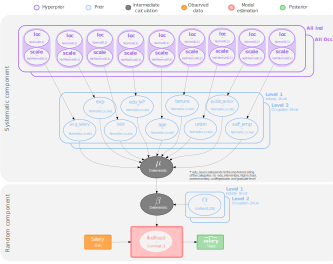
\includegraphics[width=0.95\textwidth]{./images/hierarchical_graph.png}
                \captionsetup{labelformat=empty}
                \setlength{\abovecaptionskip}{-2pt} % Reduces the space above the caption
                \caption{\fontsize{8pt}{8pt}\selectfont \textbf{\textit{Proposed salary model}}}
            \end{figure}
    \end{columns}
\end{frame}

\begin{frame}{3. Predicting salaries in ILUTE}{Results - Aggregated level (GTA)}
    \vspace*{-20pt}
    \begin{columns}
        \column{0.35\textwidth}
            \begin{itemize}
                \setlength{\itemsep}{10pt} % Adjust the item separation
                \item \fontsize{9pt}{9pt}\selectfont Annual salaries are \textbf{positive} and \textbf{right skewed}.
                \item \fontsize{9pt}{9pt}\selectfont The proposed model resembles the observed distribution by using the \textbf{Gamma random component}.
            \end{itemize}
        \column{0.7\textwidth}
            \begin{figure}
                \centering
                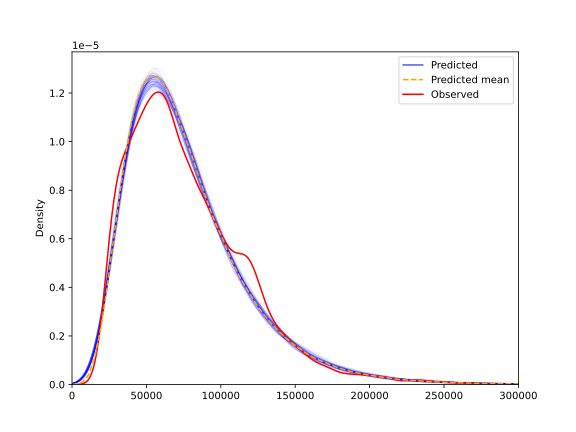
\includegraphics[width=0.85\textwidth]{./images/salary.png}
                \captionsetup{labelformat=empty}
                \setlength{\abovecaptionskip}{5pt} % Reduces the space above the caption
                \caption{\fontsize{8pt}{8pt}\selectfont \textbf{\textit{Observed and predicted annual salary distribution for the GTA}}}
            \end{figure}
    \end{columns}
\end{frame}

\begin{frame}{3. Predicting salaries in ILUTE}{Results - Aggregated level (Industry)}
    \vspace*{-23pt}
    \begin{figure}
        \centering
        \includegraphics[width=0.80\textwidth]{./images/salary_ind.png}
        \captionsetup{labelformat=empty}
        \setlength{\abovecaptionskip}{-2pt} % Reduces the space above the caption
        \caption{\fontsize{8pt}{8pt}\selectfont \textbf{\textit{Observed and predicted annual salary distribution by industry for the GTA}}}
    \end{figure}
\end{frame}

\begin{frame}{3. Predicting salaries in ILUTE}{Results - Aggregated level (Occupation)}
    \vspace*{-23pt}
    \begin{figure}
        \centering
        \includegraphics[width=0.80\textwidth]{./images/salary_occ.png}
        \captionsetup{labelformat=empty}
        \setlength{\abovecaptionskip}{-2pt} % Reduces the space above the caption
        \caption{\fontsize{8pt}{8pt}\selectfont \textbf{\textit{Observed and predicted annual salary distribution by occupation for the GTA}}}
    \end{figure}
\end{frame}

\begin{frame}{3. Predicting salaries in ILUTE}{Results - Disaggregated level (Worker)}
    \vspace*{-18pt}
    \begin{figure}
        \centering
        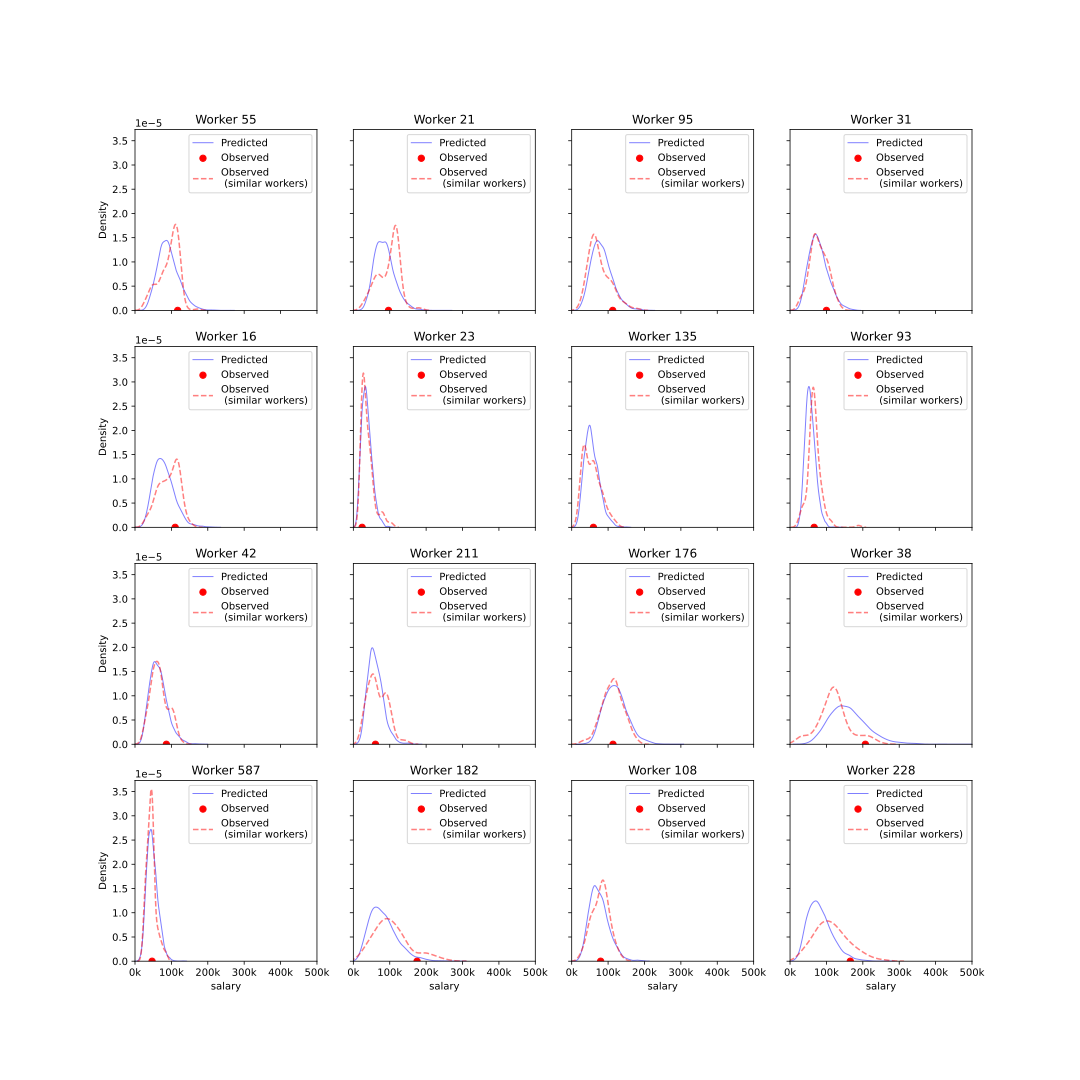
\includegraphics[width=0.90\textwidth]{./images/workers.png}
        \captionsetup{labelformat=empty}
        \setlength{\abovecaptionskip}{-2pt} % Reduces the space above the caption
        \caption{\fontsize{8pt}{8pt}\selectfont \textbf{\textit{Observed and predicted salaries for randomly selected workers}}}
    \end{figure}
\end{frame}


\begin{frame}{4. Conclusions}
    \begin{itemize}
        \setlength{\itemsep}{10pt} % Adjust the item separation
        \item \fontsize{9pt}{9pt}\selectfont Considering the hierarchical structure of the labour market has several advantages in the proposed model:
        \begin{itemize}
            \setlength{\itemsep}{10pt} % Adjust the item separation
            \item \fontsize{9pt}{9pt}\selectfont Improves the \textbf{prediction accuracy} of salaries by sharing information across industries and occupations.
            \item \fontsize{9pt}{9pt}\selectfont Enhances the \textbf{robustness} by reducing the effect of outliers \textit{(Shrinkage effect)}.
            \item \fontsize{9pt}{9pt}\selectfont Both \textbf{information sharing} and \textbf{shrinkage effect} reduces the risk of \textbf{overfitting}.
        \end{itemize}
        \item \fontsize{9pt}{9pt}\selectfont The \textbf{Gamma random component} allows the model to capture the \textbf{right skewness} of the observed salary distribution.
        \item \fontsize{9pt}{9pt}\selectfont Replacing point estimates with \textbf{probability distributions} might improve the interactions within the ILUTE labour market module.
    \end{itemize}
\end{frame}


{
\setbeamercolor{background canvas}{bg=blue}
\begin{frame}
    \begin{center}
        \textcolor{white}{{\fontsize{22pt}{14pt}\selectfont \textbf{Questions?}}}\\
        \vspace{20pt}
        \textcolor{white}{{\fontsize{14pt}{10pt}\selectfont \textsl{Thank you for your attention!}}}
    \end{center}
\end{frame}
}
\end{document}